\documentclass[colorlinks=true,pdfstartview=FitV,linkcolor=blue,
            citecolor=red,urlcolor=magenta]{basedoc}

\usepackage{graphicx}
\usepackage{amssymb}
\usepackage{amsmath}
\usepackage{longtable}
\usepackage{rotating}
\usepackage{float}
\usepackage[usenames,dvipsnames]{color}
\usepackage{fancyhdr}
\usepackage{subfigure}
\usepackage{hyperref}
\usepackage{amsmath}
\usepackage{cleveref}

\title{Experimental Methods for Determining Refraction Indices and Critical Angles of Various Acrylic Glass Media}
\author{Jorge Ramirez \\
Professor Ellen Williams, Abish Dev}


\begin{document}

  \begin{abstract}
    Two experimental methods were used to determine the indices of refraction and critical angles in acrylic glass media. The first method was conducted on a semi-circle glass prism, and the second method was conducted on a rectangular glass prism, both of thickness $10.51 \pm 0.05$mm.
    \\
    \indent The first method measured the critical angle and index of refraction by visually determining the rotation angle at which the incident laser beam was totally internally reflected. This angle was measured from the normal, and was measured in the CW and CCW directions to be $42.3^{\circ} \pm 0.35^{\circ}$ and $42.4^{\circ} \pm 0.35^{\circ}$ respectively. The indices of refraction were then calculated to be $1.486 \pm 0.35$ and $1.483 \pm 0.35$.
    \\
    \indent The second method measured the displacement in the transmitted laser beam as the rectangular prism was rotated in increments of $10^{\circ}$ in the range of $\pm50^{\circ}$. The displacement in the transmitted beam from the incident beam was then used to calculate that angle's index of refraction, and then the final value for the index of refraction for the prism was calculated from a linear fit on the data set to obtain $n_2 = 1.5002 \pm 0.0038$.

  \end{abstract}


\section{Introduction}
  This study was conducted with the intent to test experimental methods to measure the the indices of refraction of geometric acrylic glass media commonly found in undergraduate laboratories. The indices of refraction were calculated using Snell's Law which governs the behavior of light rays passing through mediums with different indices of refraction. The equation used is shown below.

    \begin{equation} \label{eq:snell}
      n_1 sin(\theta_1) = n_2 sin(\theta_2)
    \end{equation}

  In both experiments, $n_1$ was the index of refraction of the glass prism, and $\theta_1$ was the calculated angle of refraction which can be seen in the figure below. $n_2$ was set to be the index of refraction of air, close to 1, and $\theta_2$ was the angle of the incident beam measured to the normal of the surface.


    \begin{figure}[!h]
      \begin{center}
      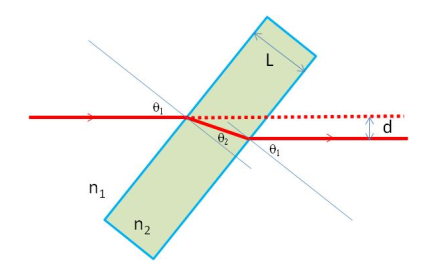
\includegraphics[width=3in]{resources/snells_law.png}
      \caption{The incident beam approaches from the left, and is displaced a distance $d$. Inside the acrylic glass, the beam is deflected by the angle of refraction $\theta_2$ (Eno, 2019)}
      \label{fig:snellslaw}
      \end{center}
    \end{figure}

  In the first method, the study sought to measure the critical angle experimentally and then use equation (2) to calculate the index of refraction of the acrylic glass, using a well known approximation that $n_2 \approx 1$.

    \begin{equation} \label{eq:snell_2}
      n_2 = \frac {sin(\theta_1)} {sin(\theta_2)}
    \end{equation}

  In the second method, the study sought to measure the index of refraction by measuring the displacement d for various incident angles $\theta_1$, and then using this measured value of d in equations (3-5). (Eno, 2019)

  \begin{equation} \label{eq:distance_d_1}
    d = \frac {L sin(\theta_1 - \theta_2 ))} {cos(\theta_2)}
  \end{equation}

  \begin{equation} \label{eq:distance_d_2}
    \frac {d} {L} = \frac {sin(\theta_1) cos(\theta_2 ) - cos(\theta_1) sin(\theta_2 )} {cos(\theta_2 )}
  \end{equation}

  \begin{equation} \label{eq:distance_d_3}
    \frac {sin(\theta_1) - \frac {d} {L}} {cos(\theta_1)} = tan(\theta_2 )
  \end{equation}

  With this angle of refraction $\theta_2$, the study then calculated the index of refraction using equation (6). (Eno, 2019).

  \begin{equation} \label{eq:ind_refr_ang_refr}
      n^2 = sin^2 \theta_1 \ [1 + \left[ \frac {cos\theta_1} {sin(\theta_1) - \frac{d}{L} } \right] ^2 ]
  \end{equation}


\section{Equipment and Procedures}

  The optical bench was setup with a 635nm coherent laser and rotating mount for the prisms to be locked in place. The mount allowed for precise rotations using a vernier scale which gave a precision of $\pm0.1^{\circ}$. At the far end of the bench was a motor-mounted photodiode, with an adjustable iris that was set to give as small of an aperture as possible in order to accurately record the transmitted laser profile. For all measurements the gain was set to give as high of a reading as possible without oversaturating the photodiode, whose maximum input voltage was $10$V.

    \begin{figure}[!h]
      \begin{center}
      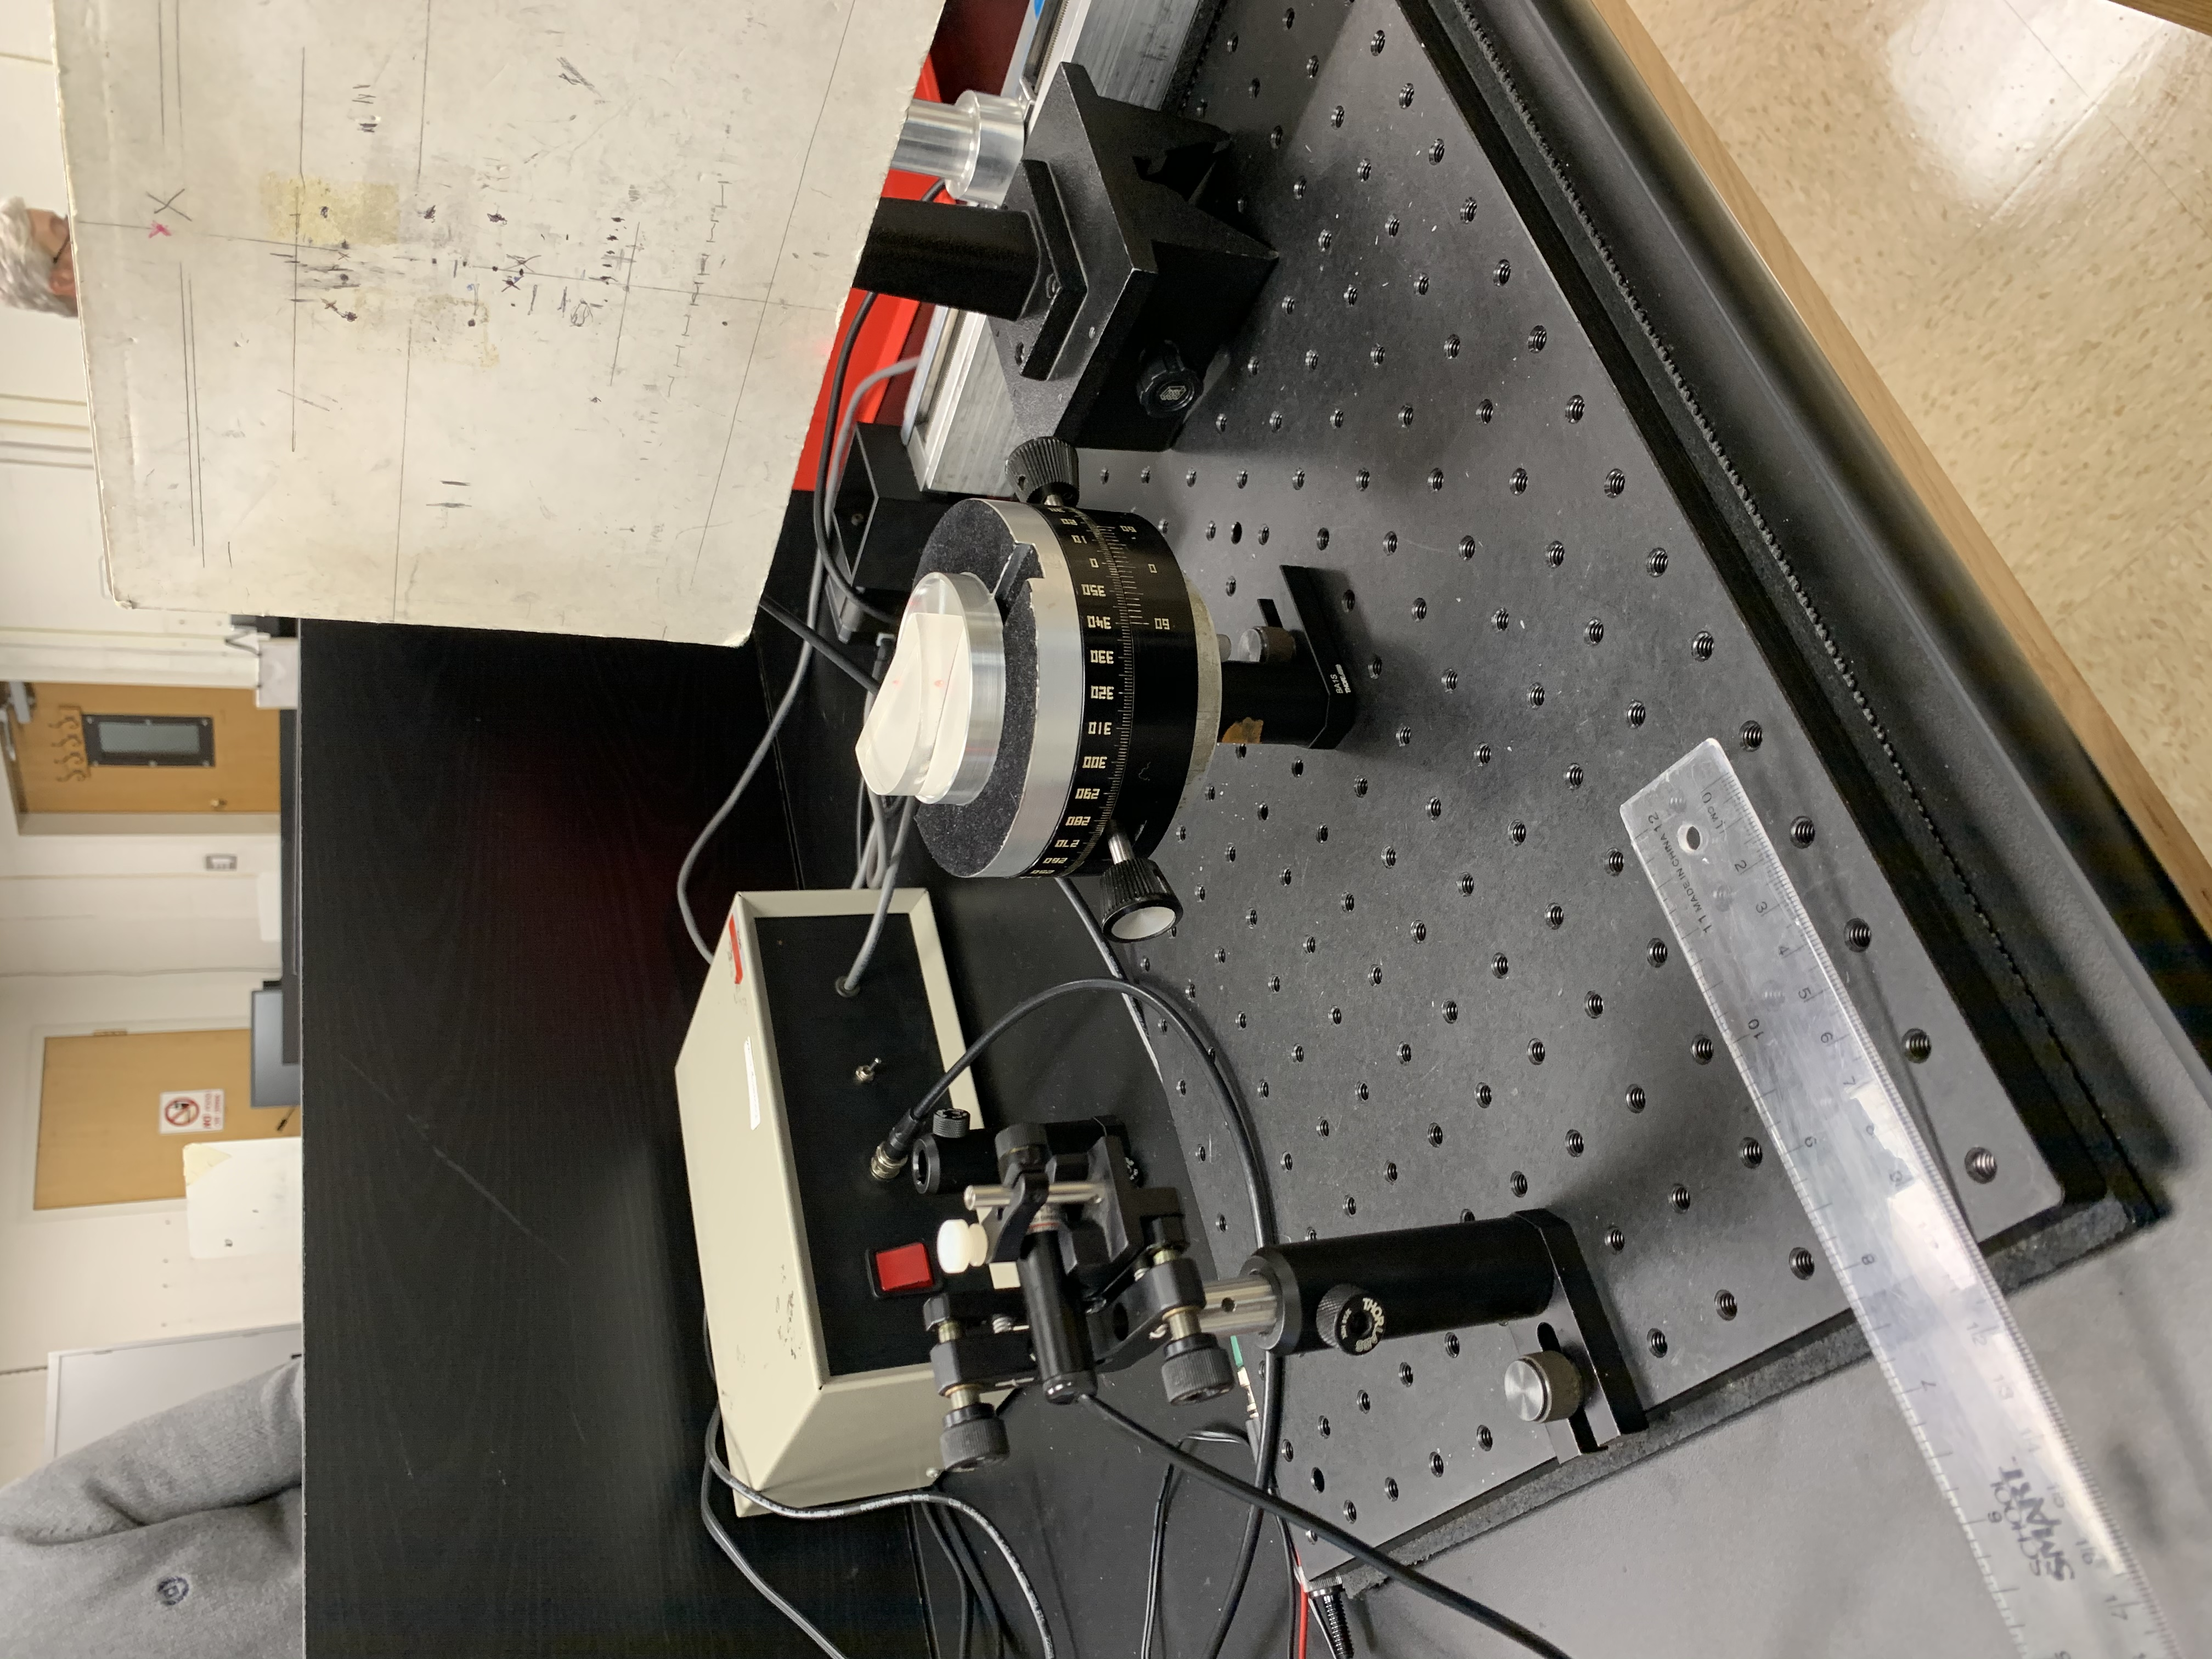
\includegraphics[angle=270,width=3in]{resources/prism_mount.jpeg}
      \caption{The rotating mount can be seen in the center of the optical bench, with the laser to its left and the stationary blocked used to track the beam at various locations on the right.}
      \label{fig:prism_mount}
      \end{center}
    \end{figure}


  The mount to hold the acrylic glass prisms was aligned by using the reflected beam off of the prism and aligning it back into the laser source. This alignment was done relative to the 0$^{\circ}$ marking on the mount itself. This ensured for both methods that the 0$^{\circ}$ reference angle was truly normal to the surface of the prism, and thus all equations used were valid. The figure above shows the aligned prism mount.

  The data was collected using a Matlab script interfacing with the photodiode through a ADC known as LabJack. Several Matlab scripts were used to perform functions such as probing the photodiode voltage, translating the photodiode, and collecting data based off of a given range of positions to scan through with the photodiode.


\section{Data Analysis}



\section{Sources of Uncertainty}

  Since the largest uncertainties in this experiment were going to be from alignment issues, several procedures were put in place to minimize the error in alignment. The laser beam needed to be at 0$^{\circ}$ inclination and 0$^{\circ}$ azimuth. These two 0$^{\circ}$ angles were alligned to satisfactory precision by using a stationary block to mark the position of the beam $1$ cm away from the source. The stationary block was then moved to the far end of the optical bench, and the beam was aligned to that same mark to ensure a horizontal beam relative to the bench itself, and that the beam was not rotated to the left or right. The uncertainty associated with this process was estimated to be about $\sigma_{\theta_1} = \pm 0.5^{\circ}$.

  For the first experimental method, a semi-circular prism was placed onto the mount. The critical angle was defined to be the angle at which the intensity of the transmitted beam drops to zero and the beam is totally internally reflected, however there was the issue of making the judgment call as to what value to assign to the critical angle. The intensity of the transmitted beam fell off rather than disappearing instantaneously. In order to minimize the uncertainty in the reported value, three separate angles were recorded for medium, low, and zero intensity transmitted beam. The critical angle was then taken to be the average of these values and the uncertainty below.

  \begin{equation} \label{eq:sigma_theta_c}
      \sigma_{\theta_c} = \frac {\text{stdev}(\theta_{c1}, \theta_{c2}, \theta_{c3})} {\sqrt{3}}
  \end{equation}



  The value of the index of refraction for each angle was expected to vary somewhat greatly due to hidden imperfections in the acrylic glass. Different incident angles led to different path lengths for the internal beam, and thus each beam would experience a varying amount of imperfections leading to noise in the collected data. This noise was reduced by repeating for many angles and then using a linear fit on equation (1).

  \begin{figure}[!h]
    \begin{center}
    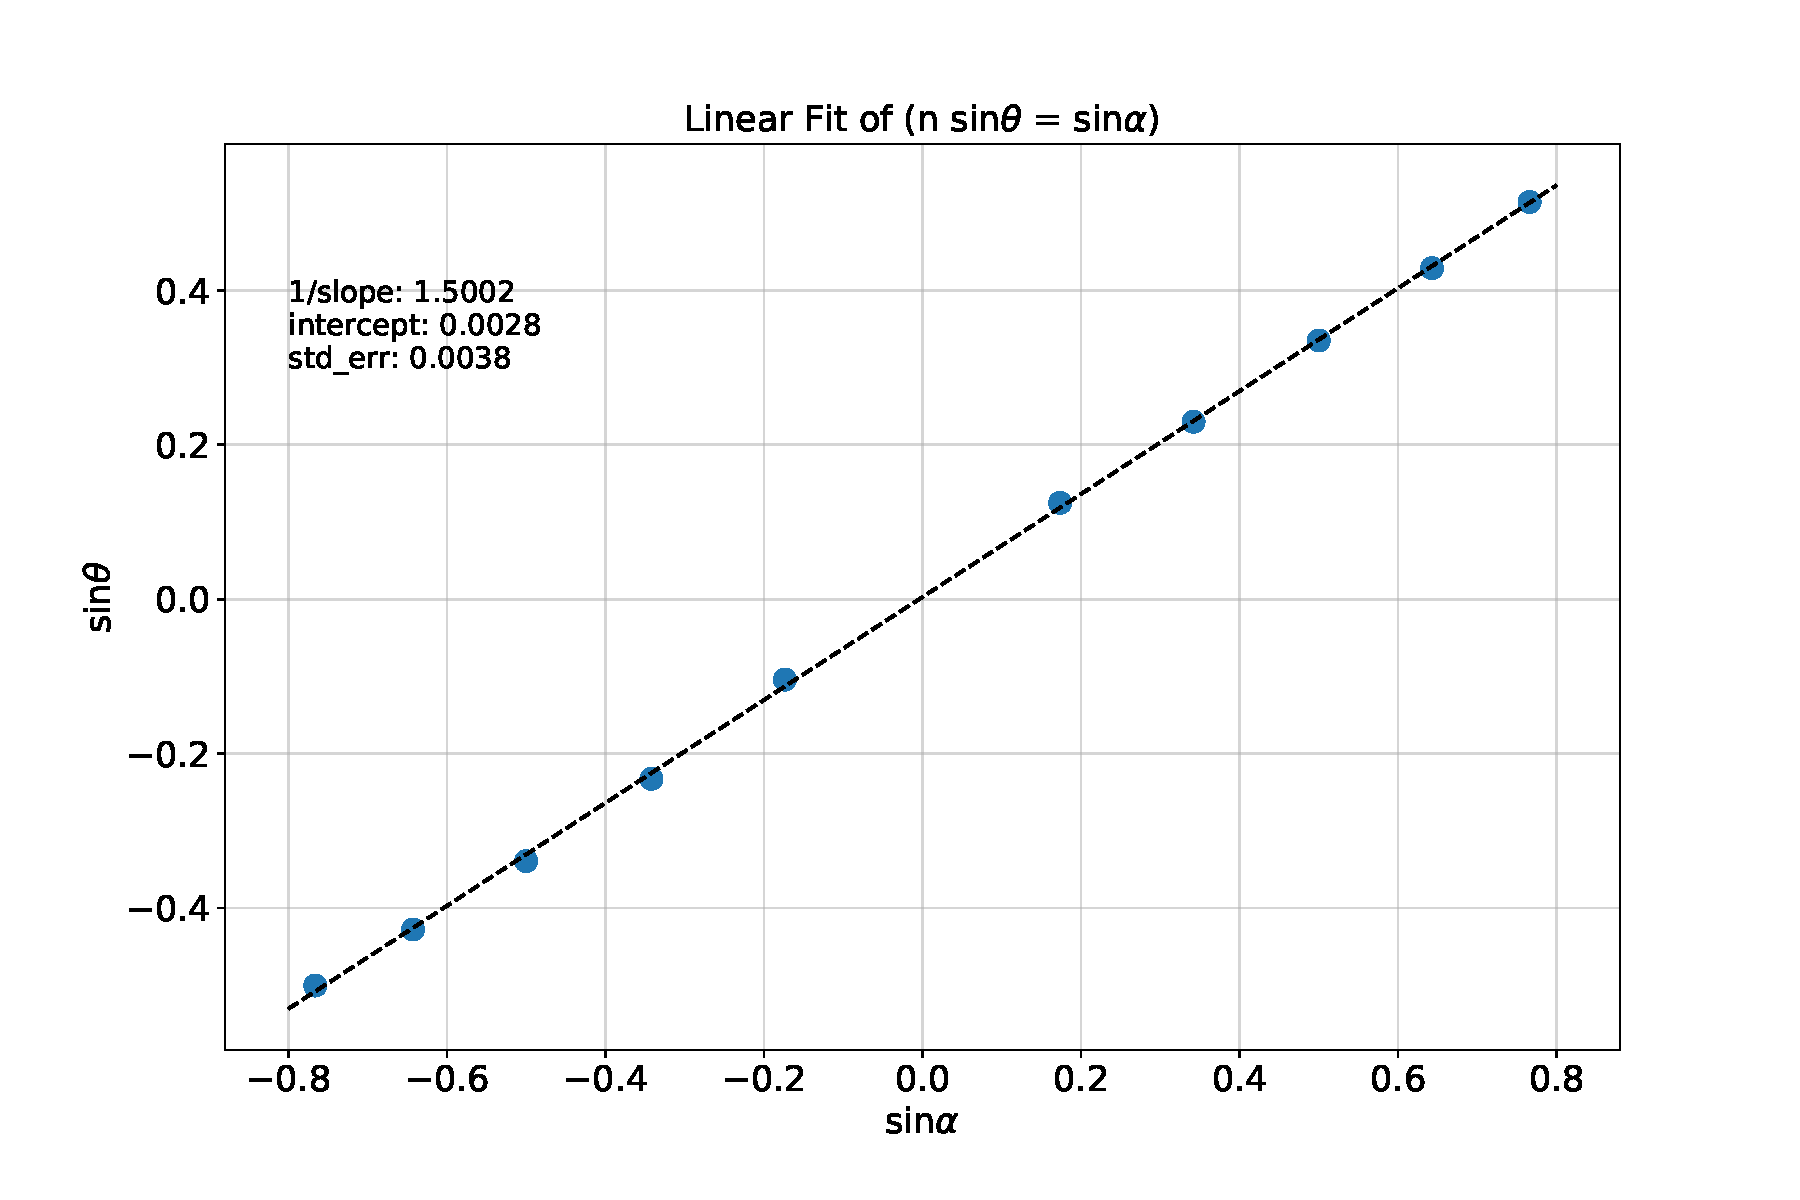
\includegraphics[width=6in]{resources/LinearFit.pdf}
    \caption{\theta refers to \theta_1, the angle of incidence, and \alpha refers to \theta_2, the angle of refraction. Although each data point had intrinsic noise due to the imperfections in the acrylic glass, this linear fit gave the final reported value for the index of refraction to be $n_1 = 1.5002 \pm 0.0038$.}
    \label{fig:lin_fit_snell}
    \end{center}
  \end{figure}

\section{Conclusions}
  The immediate future work involves improvingargins of error.



\begin{thebibliography}{9}

  \bibitem{GW Falloff}
    Eno, C. Sarah. Upadhyaya, Arpita. Williams, Ellen. Lab Manual ``PHYS 375 - Experiment I: Refraction and Reflection.'' February 10, 2020.


\end{thebibliography} %Must end the environment


\appendix \clearpage

\section{Data Analysis Code} \label{appendix:a}

  This is the code used to create a virtual two mirror cavity.1
    \begin{verbatim}
      #our two mirror cavity

      s space2 0.037 1 n4 n5
      m mirror2 0.999 0.001 0 n5 n6
    \end{verbatim}



\section{Matlab Code} \label{appendix:B}

  This is the code used to create a virtual two mirror cavity.1
    \begin{verbatim}
      #our two mirror cavity

      s space2 0.037 1 n4 n5
      m mirror2 0.999 0.001 0 n5 n6
    \end{verbatim}



\end{document}
